\section{基于RDMA的对象传输机制实现}

\subsection*{架构分析}
\begin{frame}
	\frametitle{基于RDMA的对象传输架构分析}

	\vspace{-1.6em}
	\begin{columns}[t]
		\column{0.47\textwidth}
		\begin{block}{双边通信协议}
			\begin{itemize}
				\item 预注册的发送/接收缓冲区
				\item 无需重复注册
			\end{itemize}
		\end{block}
		\column{0.47\textwidth}
		\begin{block}{单边通信协议}
			\begin{itemize}
				\item 原地注册的缓冲区
				\item 零拷贝
			\end{itemize}
		\end{block}
	\end{columns}

	\begin{figure}
		\centering
		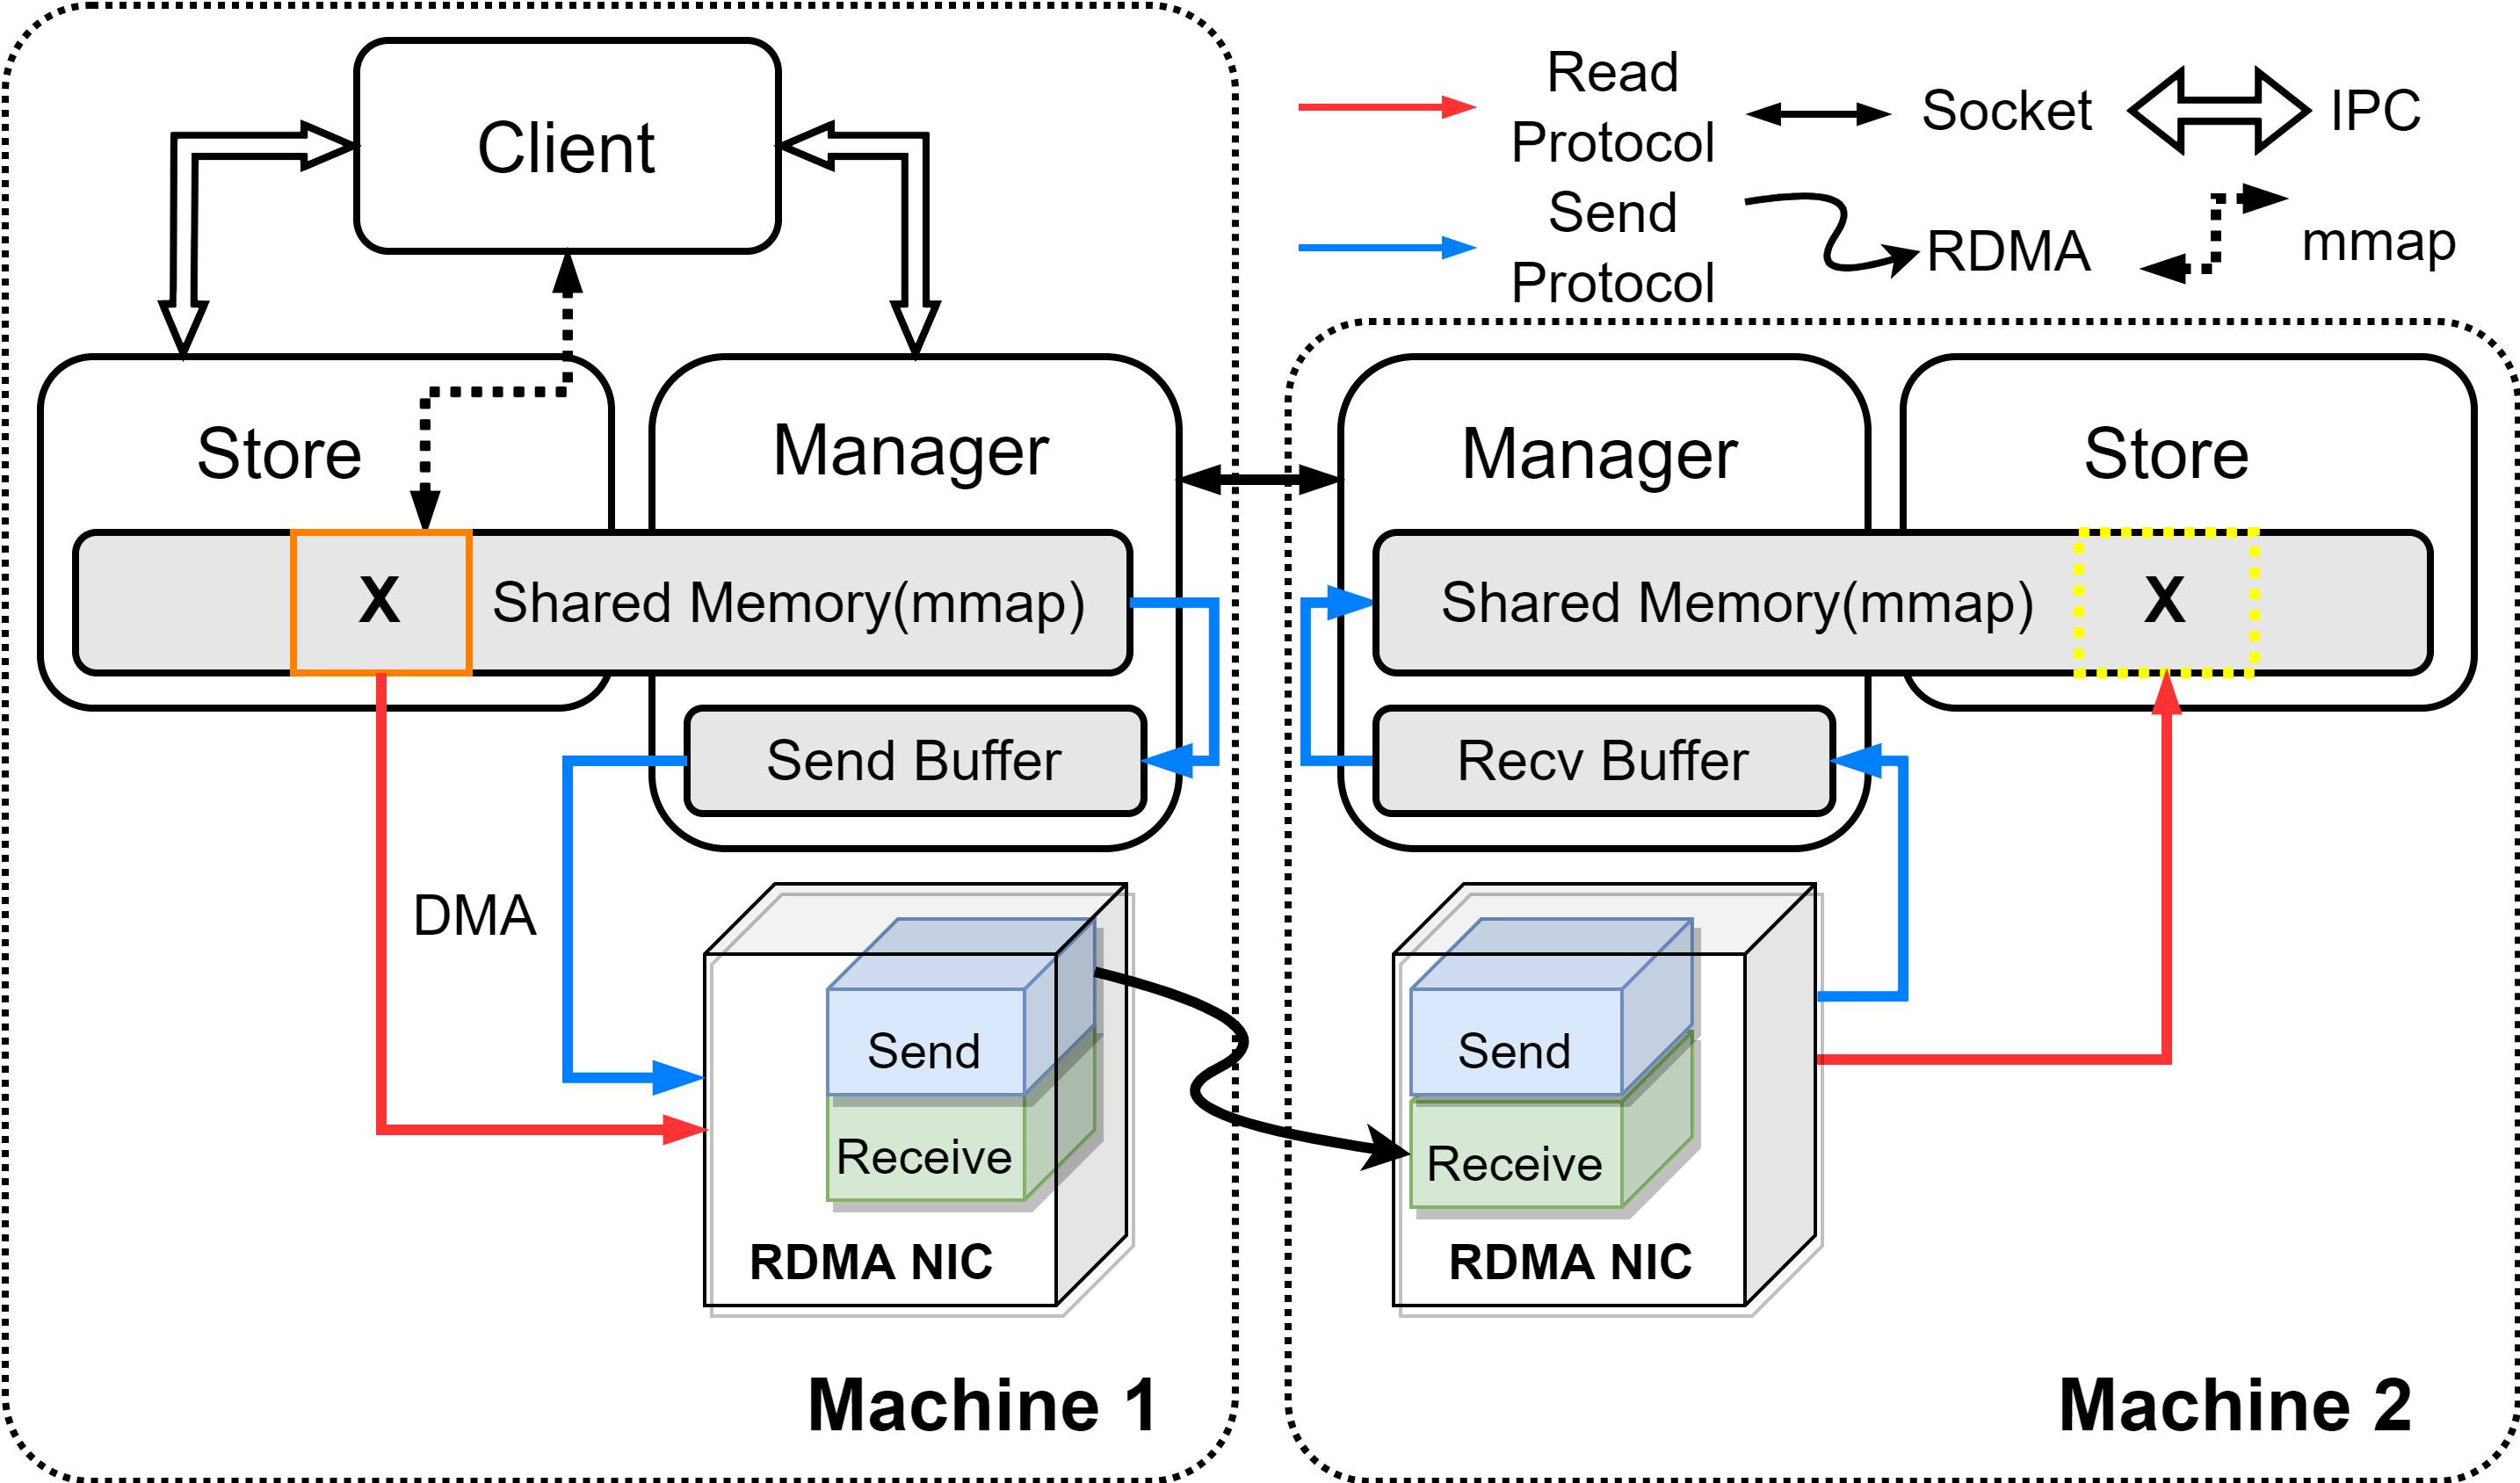
\includegraphics[width=0.65\textwidth]{image/chap03/rdma_arch.png}
		\caption{基于RDMA的对象传输架构}
	\end{figure}

\end{frame}

\subsection*{协议分析}
\begin{frame}
	\frametitle{双边传输协议}
	\begin{columns}[onlytextwidth]
		\column{0.4\textwidth}
		\begin{block}{消息}
			\begin{itemize}
				\item PLASMA\_TRANSFER:\\发起对象X的传输
				\item PLASMA\_DATA:\\返回X的元数据
				\item data:对象数据
			\end{itemize}
		\end{block}
		\begin{block}{分析}
			\begin{itemize}
				\item 清空缓冲后同步(ACK)
				\item 无内存注册
				\item 适合传输小对象
			\end{itemize}
		\end{block}
		\column{0.57\textwidth}
		\begin{figure}
			\centering
			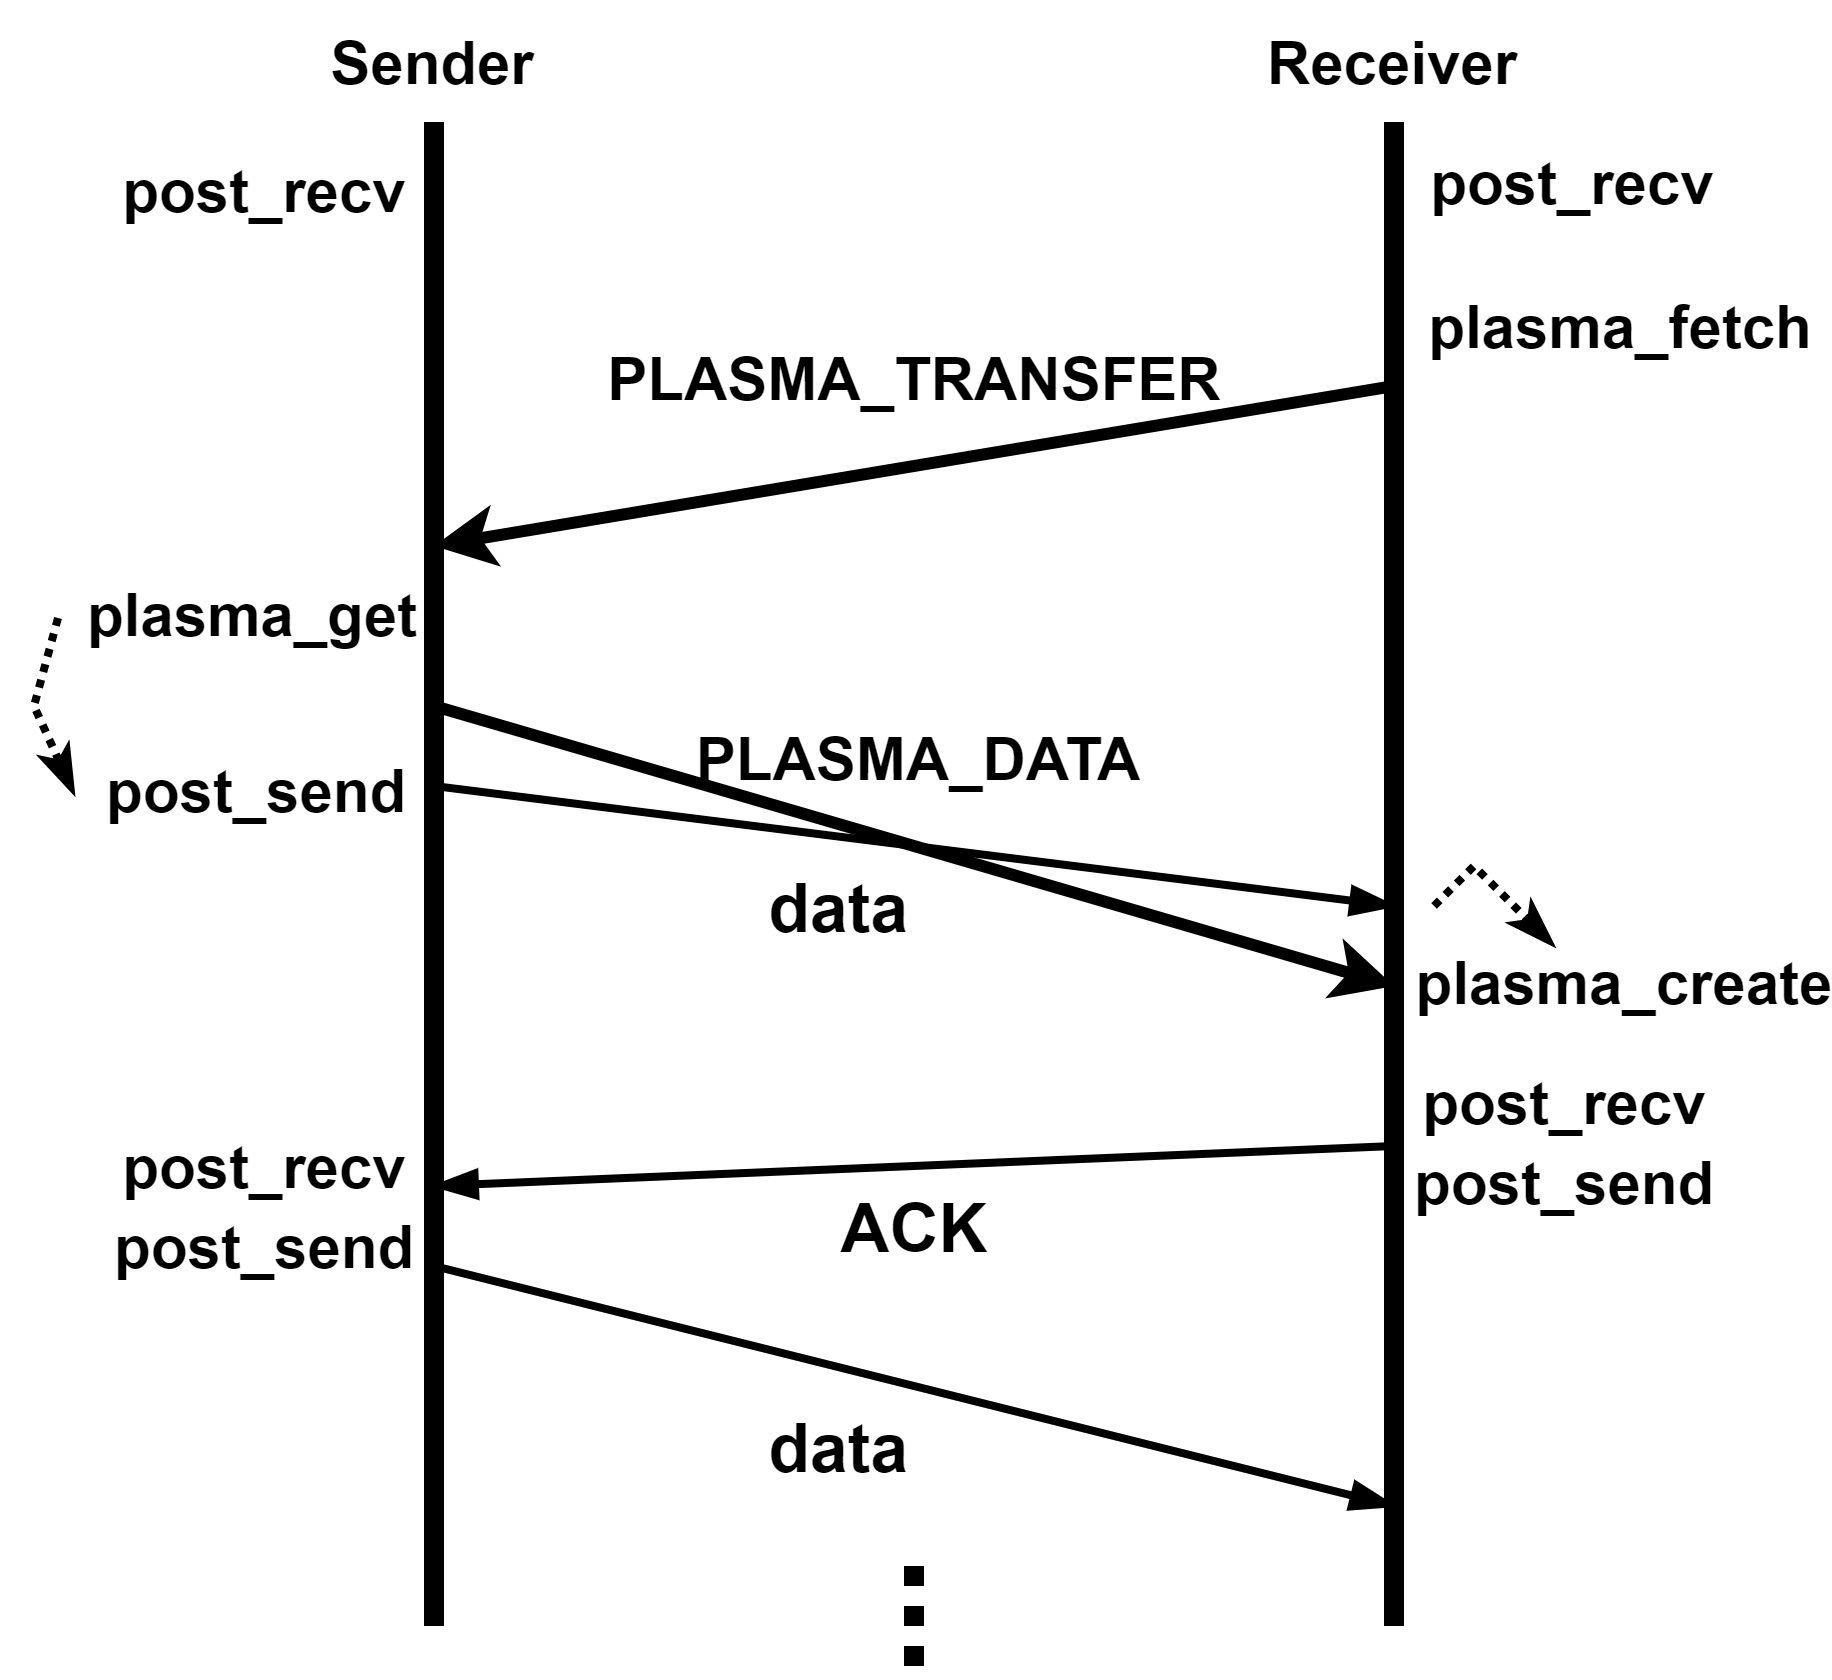
\includegraphics[width=\textwidth]{image/chap03/send_protocol.png}
			\caption{双边传输协议}
		\end{figure}
	\end{columns}
\end{frame}

\begin{frame}
	\frametitle{单边传输协议}
	\begin{columns}[onlytextwidth]
		\column{0.4\textwidth}
		\begin{block}{消息}
			\begin{itemize}
				\item PLASMA\_DATA\\加入远端地址信息
				\item Read:单边读
			\end{itemize}
		\end{block}
		\begin{block}{分析}
			\begin{itemize}
				\item 即时注册/释放对象地址
				\item 零内存拷贝
				\item 适合传输大对象
			\end{itemize}
		\end{block}
		\column{0.57\textwidth}
		\begin{figure}
			\centering
			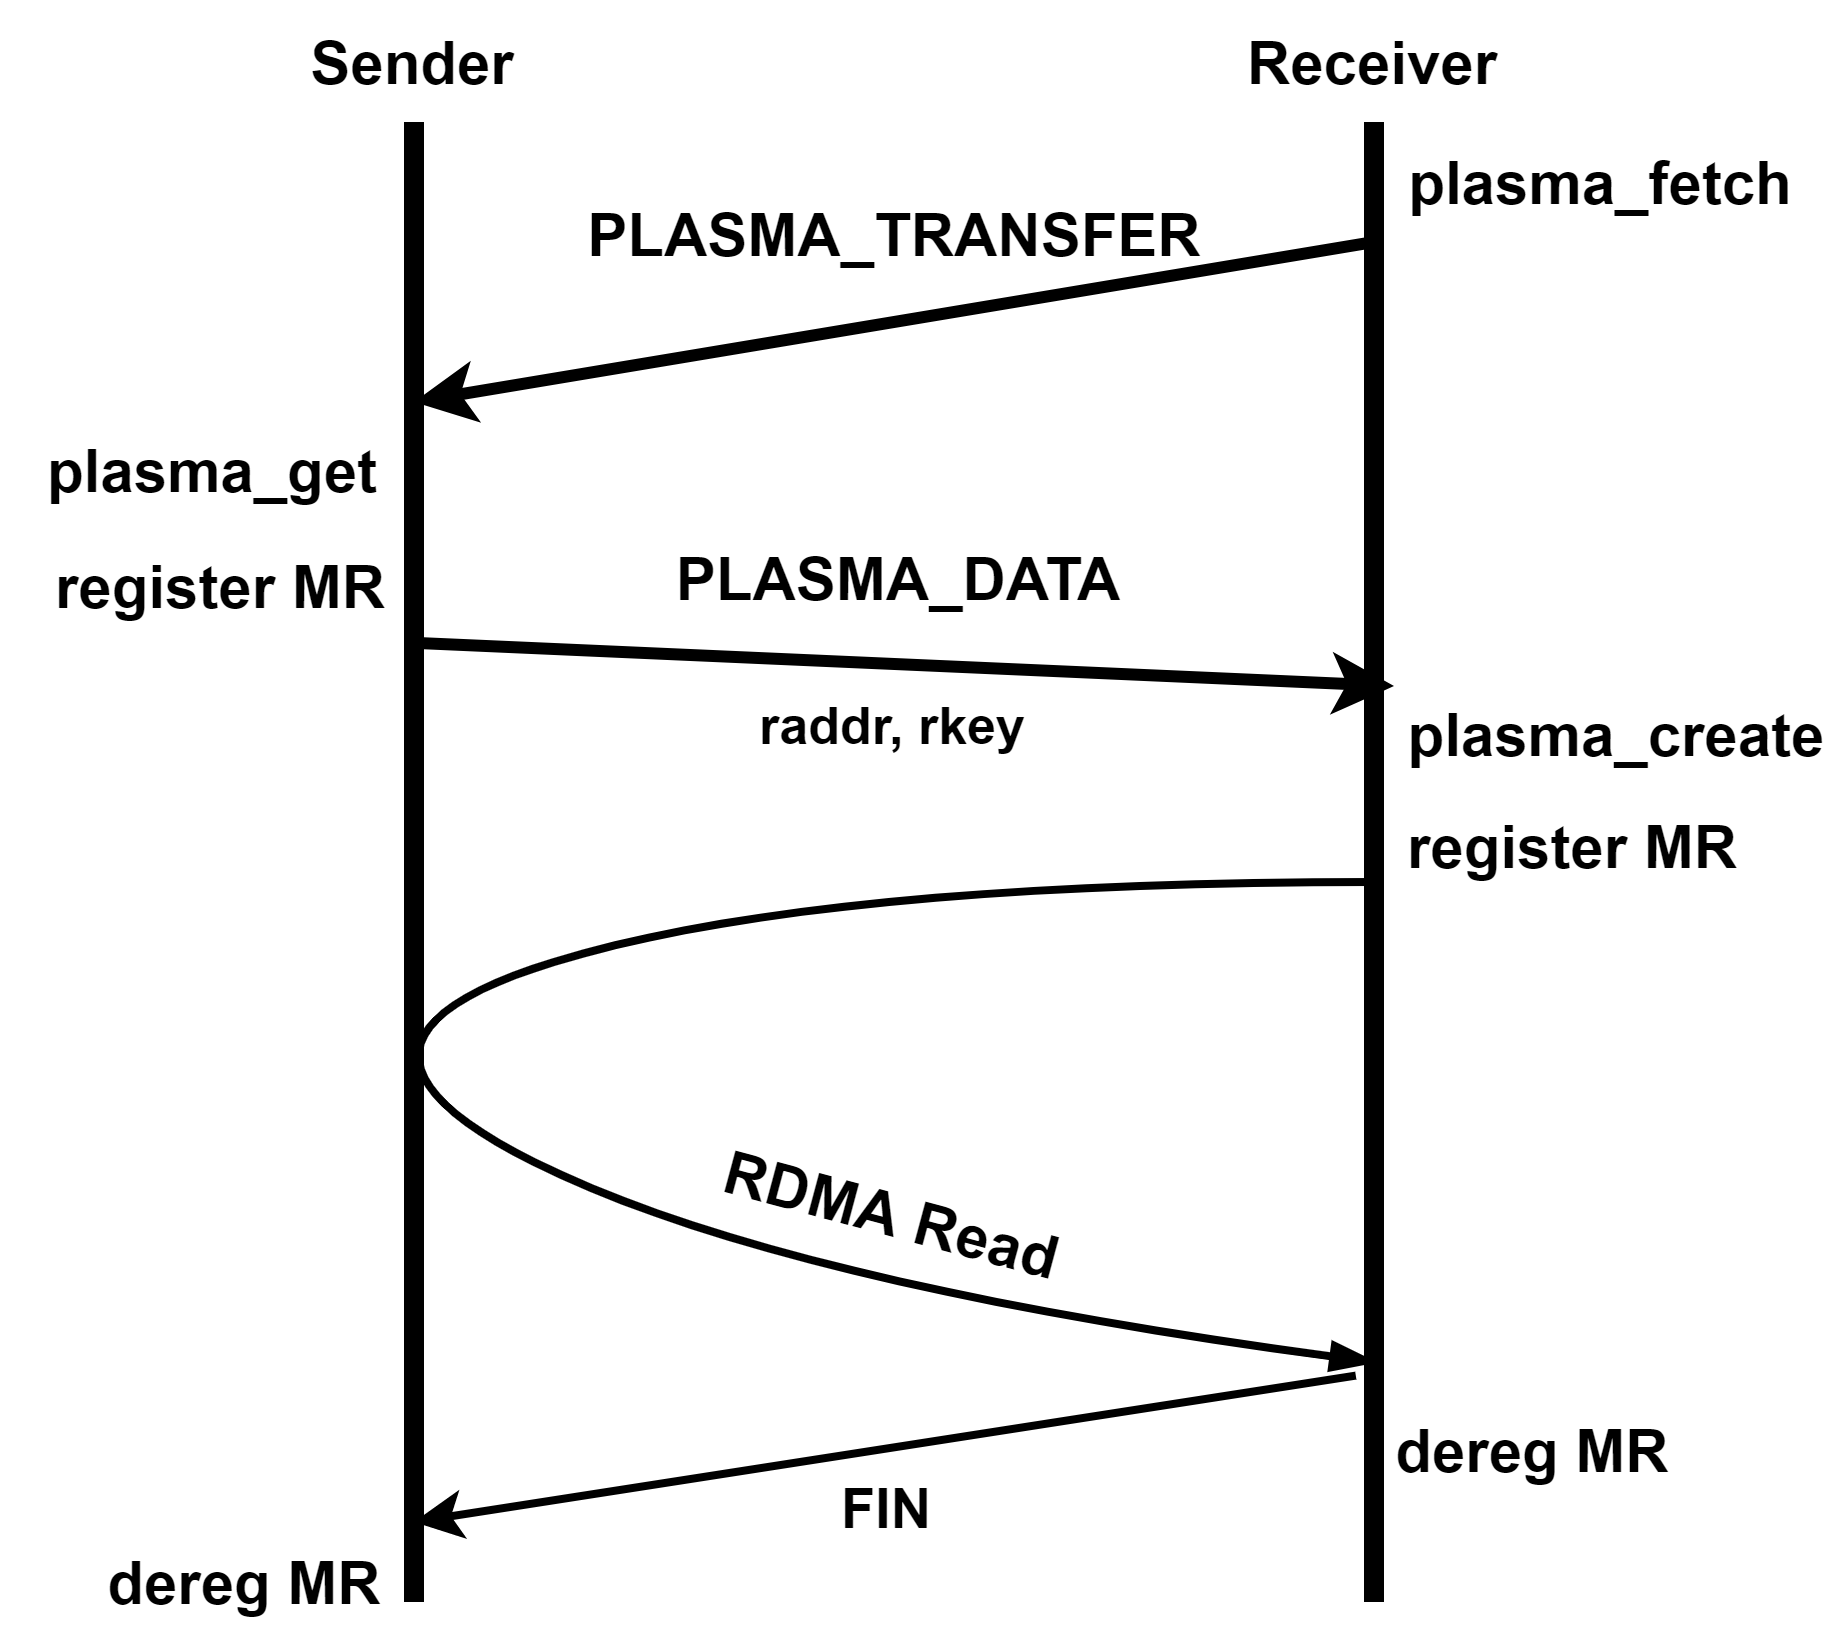
\includegraphics[width=\textwidth]{image/chap03/read_protocol.png}
			\caption{单边传输协议}
		\end{figure}
	\end{columns}
\end{frame}